
\def\colegio{Colegio Latinoamericano de Integración}
\def\titulo{Guía}
\def\subtitulo{Ecuaciones}
\documentclass[options]{plantilla-material-v1}

\begin{document}
\section{Operatoria algebraica}

Reduce las siguientes expresiones algebraicas.
\begin{ejercicios}[resume](1)
  \ejercicio $3x +6y +2x -4y$
  \ejercicio $6m -17n +8n +7m -2n$
  \ejercicio $2x +6y +3x^2 +5x +5x^2$
  \ejercicio! $4a -2ab^3 +3b +5a +8ab^3$
  \ejercicio $2ab + 2b -(4ab+5b)$
  \ejercicio $3b + 3xy -(-6b+8xy)$
\end{ejercicios}

Considera las siguientes igualdades y luego calcula.
\figuraTriple{$A=m+n$}{$B=2m-n$}{$C=4m-3n$}
\begin{ejercicios}[resume](2)
  \ejercicio $A+B$
  \ejercicio $A+B+C$
  \ejercicio $A-B$
  \ejercicio $B-A$
  \ejercicio $A-(B+C)$
  \ejercicio $B-(A+C)$
\end{ejercicios}

Desarrolla los siguientes productos.
\begin{ejercicios}[resume](1)
  \ejercicio $3\cdot(a+d)$
  \ejercicio $b\cdot(3d-f)$
  \ejercicio $2b\cdot(l+3t-8b)$
  \ejercicio $5t\cdot(8d-2r+d^5)$
  \ejercicio $(2+f)\cdot(g+3h)$
  \ejercicio $(r+5t)\cdot(k-g)$
  \ejercicio $(m-n)\cdot(q-p+1)$
  \ejercicio $t^2\cdot(5d-2l+11+t^2)$
\end{ejercicios}

Considera las siguientes igualdades y luego calcula.
\figuraTriple{$A=m+1$}{$B=2m-3$}{$C=4m-3n$}
\begin{ejercicios}[resume](2)
  \ejercicio $2A$
  \ejercicio $5B$
  \ejercicio $A\cdot B$
  \ejercicio $B\cdot C$
  \ejercicio $2\cdot(B+C)$
  \ejercicio $6\cdot(A-C)$
\end{ejercicios}

Resuelve las siguientes multiplicaciones de expresiones algebraicas. Luego, reduce los
términos semejantes.

\begin{ejercicios}[resume](1)
  \ejercicio $5x\cdot8x$
  \ejercicio $(8-4y^2+3x^2)\cdot 10xy$
  \ejercicio $(-x^2+2x)\cdot(5x-0.5x^2)$
  \ejercicio $(11mn+3m^2n)\cdot(-4mn^2-mn+0.25)$
  \ejercicio $\left(\dfrac{1}{2}xy+\dfrac{1}{4}\right)\cdot
    \left(\dfrac{3}{4}x^2-\dfrac{1}{2}xy\right)$
  \ejercicio $\left(\dfrac{1}{5}a-\dfrac{3}{2}b-2\right)\cdot
    \left(-2a-\dfrac{1}{7}b+1\right)$
  \ejercicio $\left(\dfrac{2}{3}x^3y-\dfrac{4}{7}xy\right)\cdot
    \left(\dfrac{5}{8}xy-\dfrac{6}{5}x^2y\right)$
  \ejercicio $(-4ab^2+3a^2b^2-5ab^2-2)\cdot(-6ab+5)$
\end{ejercicios}

Determina una expresión algebraica reducida para el área y perimetro de las siguientes
figuras.
\begin{ejercicios}[resume](1)
  \ejercicio
  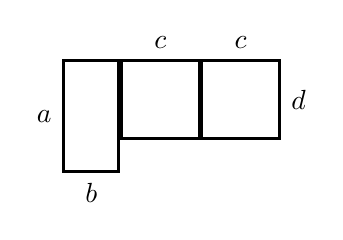
\begin{tikzpicture}[baseline=(current bounding box.north),line width=1pt]
    \node[draw,shape=rectangle,inner ysep=20,inner xsep=10] (R) {};
    \node[draw,shape=rectangle,inner sep=14,anchor=north west] (Q) at (R.north east) {};
    \node[draw,shape=rectangle,inner sep=14,anchor=north west] (QQ) at (Q.north east) {};
    \node[left] at (R.west) {$a$};
    \node[below] at (R.south) {$b$};
    \node[above] at (Q.north) {$c$};
    \node[above] at (QQ.north) {$c$};
    \node[right] at (QQ.east) {$d$};
  \end{tikzpicture}
  \ejercicio
   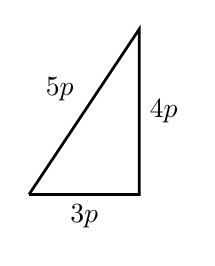
\begin{tikzpicture}[scale=0.7,baseline=(current bounding box.north),line width=1pt]
      \draw (0,0) -- (2,0) node[midway,below] {$3p$} --([turn]90:3) node[midway,right] {$4p$} -- (0,0)
        node[midway,above left] {$5p$};
   \end{tikzpicture}
\end{ejercicios}

\section{Solucionar para una incógnita}
\NewDocumentCommand{\incognita}{}{
  \tcbox[colback=black!60, colframe=black!60, coltext=white, on line, boxsep=0pt, left=2pt, right=2pt, top=2pt, bottom=2pt,width=1cm]{\bfseries ?}
}
En cada caso, determine el término que falta para que se cumpla la igualdad.
\begin{ejercicios}[resume](1)
  \ejercicio $6m+4n+\incognita + 6n = 17m +10n$
  \ejercicio $3ab + 6b + \incognita - 10b = 5ab - 4b$
  \ejercicio $4x+8y+\incognita + 5x + 7x^2 = 8x +8y +16x^2$
  \ejercicio $7a -8ab^3 +6b +5a +9ab^3 = \incognita + 6b + ab^3$
\end{ejercicios}

Determina la medida del lado desconocido en cada rectángulo considerando el área dada.
\begin{ejercicios}[resume](2)
  \ejercicio 
  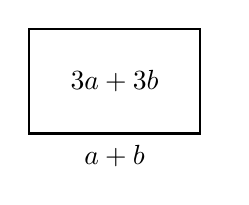
\begin{tikzpicture}[scale=0.5,baseline=(current bounding box.north),line width=1pt]
    \node[draw,shape=rectangle,name=R,inner sep=15pt] {$3a+3b$};
    \node[below] at (R.south) {$a+b$};
    \node[right] at (R.east) {\incognita}; 
  \end{tikzpicture}
  \ejercicio 
  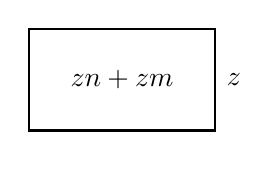
\begin{tikzpicture}[scale=0.5,baseline=(current bounding box.north),line width=1pt]
    \node[draw,shape=rectangle,name=R,inner sep=15pt] {$zn+zm$};
    \node[below] at (R.south) {\incognita};
    \node[right] at (R.east) {$z$}; 
  \end{tikzpicture}
  \ejercicio!
  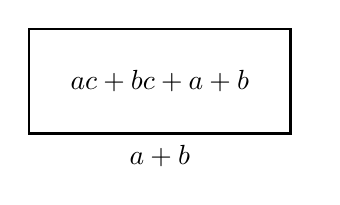
\begin{tikzpicture}[scale=0.5,baseline=(current bounding box.north),line width=1pt]
    \node[draw,shape=rectangle,name=R,inner sep=15pt] {$ac+bc+a+b$};
    \node[below] at (R.south) {$a+b$};
    \node[right] at (R.east) {\incognita}; 
  \end{tikzpicture}

\end{ejercicios}
\end{document}